\documentclass[10pt,professionalfont,utf8,presentation,compress]{beamer}

\usepackage{sty/beamer}

\uselanguage{russian}
\languagepath{russian}

\usepackage{multicol} 		% Несколько колонок
\graphicspath{{images/}}  	% Папка с картинками

\usepackage{siunitx}
\usepackage{newtxtext,newtxmath}
\usepackage{bm}

\usepackage{longtable,rotating}
\usepackage{threeparttable}

% для картинок
\usepackage{chngcntr}
%\counterwithin{figure}{section}

\setbeamerfont{author}{size=\fontsize{11pt}{12pt}}
\setbeamerfont{institute}{size=\fontsize{10pt}{11pt}}

\setbeamertemplate{theorem}[ams style]
\setbeamertemplate{theorems}[numbered]

\setbeamertemplate{caption}[numbered]

\setbeamertemplate{bibliography item}{\insertbiblabel}
\setbeamertemplate{bibliography entry article}{}
\setbeamertemplate{bibliography entry title}{}
\setbeamertemplate{bibliography entry location}{}
\setbeamertemplate{bibliography entry note}{}

\setbeamerfont{bibliography entry author}{size=\footnotesize}
\setbeamerfont{bibliography entry title}{size=\footnotesize}
\setbeamerfont{bibliography entry location}{size=\footnotesize}
\setbeamerfont{bibliography entry note}{size=\footnotesize}

\theoremstyle{definition}
\newtheorem{defn}{Определение}

\theoremstyle{plain}
\newtheorem{exmp}{Пример}


%\usetheme{Madrid}


% информация для титульника и для подписей слайдов
\title[Приложения $p$-адической арифметики]
{Приложение $p$-адической арифметики к задачам компьютерной алгебры}
\author{Шаров Александр Вадимович}
\institute{{Саратовский государственный университет} \\
    им.~Н.~Г.~Чернышевского \\[5pt]
Кафедра дискретной математики\\[5pt]
Научный руководитель: к.~ф.-м.~н., доцент Тяпаев~Л.~Б.
}
\date{18 Июня 2020 г.}


\begin{document}

\frame[plain]{\titlepage}


% Постановка задачи - обязательный слайд
\begin{frame}
    \frametitle{Цели работы}
    \Large
    \begin{enumerate}
        \item Дать алгоритмическое описание $p$-адической арифметики и реализовать библиотеку для работы с объектами компьютерной алгебры на ЯП Python с её применением.
        \item Привести примеры использования реализованной библиотеки для популярных задач физики и математики.
       	\item Провести сравнение библиотеки для работы с $p$-адической арифметикой с классическими методами.
    \end{enumerate}
\end{frame}


\begin{frame}
    \frametitle{Задачи}
    %\Large
    \begin{enumerate}
        \item Разработать классы для работы с $p$-адические числами и матрицами на ЯП Python. 
        \item Провести сравнение классических методов и однопоточной $p$-адической арифметики.
        \item Реализовать многопоточный вариант $p$-адической арифметики.
       	\item Провести сравнение библиотеки для работы с $p$-адической арифметикой с классическими методами на примере таких задач, как: вычисление определителя, решение СЛАУ И ОДУ, нахождение собственных чисел и векторов, вычисление матричной экспоненты.
    \end{enumerate}
\end{frame}


% Слайд 3
\begin{frame}
\frametitle{$p$-адические числа}

\begin{defn}
Пусть $p \in \mathbb {P}$ -- некоторое простое число. В поле $\mathbb {Q}$ введем другую норму $\norm{.}_p$ по правилу:
\begin{enumerate}
	\item $\norm{0}_p = 0$,
	\item $\norm{n}_p = p ^ {-ord_pn}$,
\end{enumerate}
\noindent где $n > 0$ - некоторое натуральное число, а $ord_pn$ - показатель степени, в которой число $p$ входит в это произведение. В этом случае норма $\norm{.}_p$ называется \mbox{$p$-адической} нормой.
\end{defn}

\begin{defn}
Пополнение поля $\mathbb {Q}$ по $p$-адической норме образует поле $\mathbb {Q}_p$ $p$-адических чисел.
\end{defn}

\end{frame}


% Слайд 4
\begin{frame}
\frametitle{$p$-адические числа}
\begin{defn}
Любое $p$-адическое число $x \ne 0$ однозначно представляется в каноническом виде

\begin{equation} \label{numbers:decomposition}
	x = p^{\gamma} \cdot (x_0 + x_1\cdot p + x_2 \cdot p^2 + \dots),
\end{equation}

\noindent где $\gamma = \gamma(x) \in \mathbb {Z}$ и $x_j$ -- целые числа, при которых $0 \le x_j \le p-1$, $x_0 > 0,$ $(j=0,1,\dots)$.
\end{defn}
\end{frame}


% Слайд 5
%\begin{frame}
%\frametitle{$p$-адические числа: пример сложения чисел}

%\begin{exmp}
%Сложить $\frac{2}{3}$ и $\frac{5}{6}$ в $\mathbb{Q}_5$.

%\noindent $5$-адическое разложение слагаемых имеет вид

%$$
%\frac{2}{3}=.4131313\dots
%$$
%$$
%\frac{5}{6}=.0140404\dots
%$$
%Выполняя сложение, получим

%$$
%\begin{tabular}{cccccccccccc}
%& + & . & 4\; & 1\; & 3\; & 1\; & 3 & 1 & 3 & \dots \\
%& = & . & 0\; & 1\; & 4\; & 0\; & 4 & 0 & 4 & \dots \\
%\hline
%& = & . & 4\; & 2\; & 2\; & 2\; & 2 & 2 & 2 & \dots
%\end{tabular}
%$$

%\noindent В свою очередь $\bigg(\frac{3}{2}\bigg)_5=.4222222\dots$
%\end{exmp}
%\end{frame}


% Слайд 6
\begin{frame}
\frametitle{$p$-адические числа: код Гензеля}
\begin{defn}
Пусть $p$-простое число, $r$-натуральное число и $\alpha=\sum\limits^{\infty}_{i=m} a_ip^i$ - $p$-адическое число ($0 \le a_i \le p, a_m \neq 0$). Кодом Гензеля $p$-адического числа $\alpha$ назовем $p$-адическое представление числа $\sum\limits_{i=m}^{r}a_ip^i$. Для кодов Гензеля будем использовать обозначение $H(p,r,\alpha)$, явно содержащее числа $p$, $r$ и $\alpha$. Упрощенный вариант будем обозначать как $H_{p,r}(\alpha)$.
\end{defn}
\end{frame}


% Слайд 7
\begin{frame}
\frametitle{$p$-адические числа: код Гензеля}
\begin{exmp}
Получить код Гензеля для разности чисел $\frac{3}{4}$ и $\frac{3}{2}$ в $\mathbb{Q}_5$.

\noindent Код Гензеля для операндов имеет следующий вид:

$$H\bigg(5,4, \frac{3}{4}\bigg)=(.\; 2\; 1\; 1\; 1)$$

$$H\bigg(5,4, \frac{3}{2}\bigg)=(.\; 4\; 2\; 2\; 2)$$


\noindent Произведем вычитание:

$$
\begin{tabular}{ccccccccccc}
& - & .\; & 2\; & 1\; & 1\; & 1\; &  \\
& = & .\; & 4\; & 2\; & 2\; & 2\; &  \\
\hline
& = & .\; & 3\; & 3\; & 3\; & 3\; &
\end{tabular}
$$

\noindent Таким образом, результатом является код Гензеля $(.\; 3\; 3\; 3\; 3)$, который представляет собой рациональное число $-\frac{3}{4}$.
\end{exmp}
\end{frame}


% Слайд 8
\begin{frame}
\frametitle{Программная реализация}
	\begin{figure}[H]
	\centerline{
\includegraphics[width=0.5\linewidth]{images/python.png}}
	\end{figure}
\end{frame}


% Слайд 9
\begin{frame}
\frametitle{Программная реализация: состав модулей библиотеки}
\begin{itemize}
\item Модуль для работы с $p$-адическими числами. Содержит базовые арифметические и алгебраические операции, а также представляет основные программные интерфейсы, например, ввод и вывод чисел в человекочитаемом формате.
\item Модуль для работы с матрицами и векторами. Предоставляет базовые операции над матрицами, а также вспомогательные функции для выполнения математических операций с использованием матричной арифметики.
\item Модуль с реализацией таких базовых алгоритмов, как вычисление определителя матрицы, решение СЛАУ методами Крамера и Гаусса, алгоритм Якоби для вычисления собственных значений и собственных векторов. Кроме того данный модуль содержит реализацию решения дифференциальных уравнений методами Эйлера и методом Рунге-Кутта четвертого порядка.
\end{itemize}
\end{frame}


% Слайд 10
\begin{frame}
\frametitle{Описание матрицы для сравнения производительности}

$A: \dim{A} = 1000$ и коэфициенты вычисляются следующим образом:

\begin{equation}
a_{i,j}=
\begin{cases}
1-\bigg(round\bigg(\frac{i-j}{n}\bigg)\bigg)^2, \; i \neq j, \\
10-round\bigg(\frac{i-j}{n}\bigg), \; i = j.
\end{cases}
\end{equation}
\end{frame}


% Слайд 11
\begin{frame}
\frametitle{Сравнение производительности: вычисление определителя}
\begin{figure}[H]
\centerline{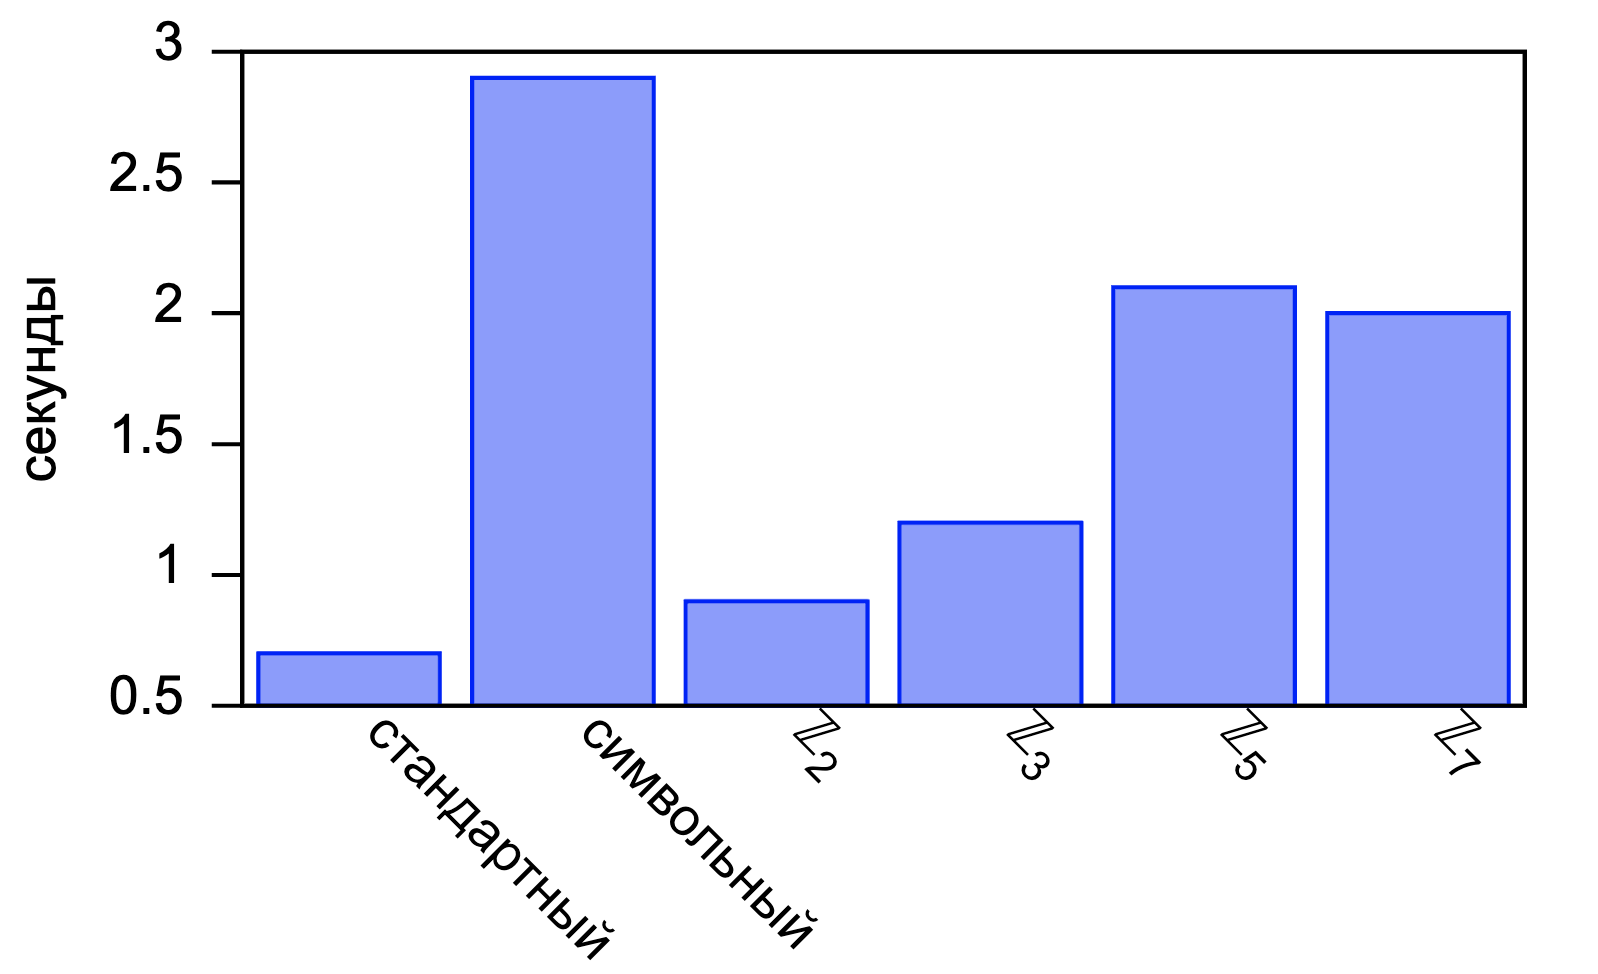
\includegraphics[width=0.95\linewidth]{../gnuplot/single/det/plot.png}}
\caption{График производительности однопоточных методов для вычисления определителя матрицы.}
\label{img:single:det:1}
\end{figure}
\end{frame}


% Слайд 12
\begin{frame}
\frametitle{Сравнение производительности: вычисление определителя}
\begin{figure}[H]
\centerline{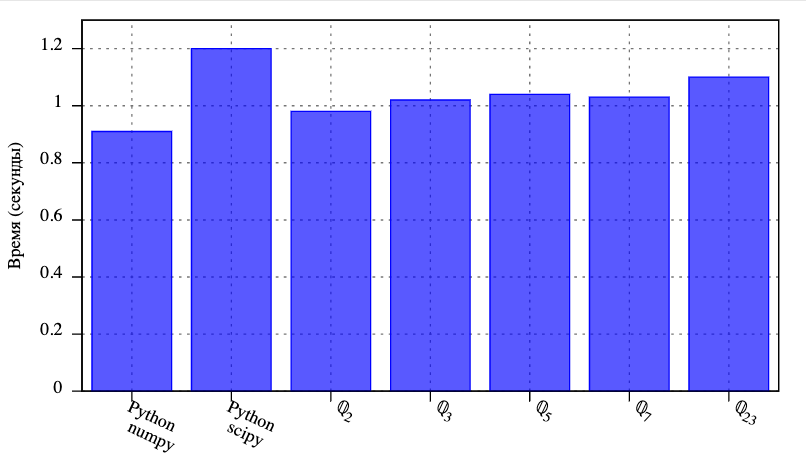
\includegraphics[width=0.95\linewidth]{../gnuplot/single/det/wosymb.png}}
\caption{График производительности однопоточных методов для вычисления определителя матрицы (без символьного метода).}
\label{img:single:det:2}
\end{figure}
\end{frame}


% Слайд 13
\begin{frame}
\frametitle{Сравнение производительности: решение СЛАУ}
Для сравнения производительности классического и $p$-адического метода решения СЛАУ решим $m$ раз систему из $n$ уравнений:

\begin{equation}
\boldsymbol{A}*\boldsymbol{X}=\boldsymbol{B},
\end{equation}

\noindent где $\boldsymbol{A}$ - матрица коэффициентов размером $n \times n$, $\boldsymbol{X}$ - вектор неизвестных и $\boldsymbol{B}$ - вектор правых частей.
Пусть коэффициенты матрицы $\boldsymbol{A}$ вычисляются следующим образом:

\begin{equation}
a_{i,j}=
\begin{cases}
\abs{1-rand(n)*round\bigg(i-j\bigg)^2}, i \neq j, \\
10, i = j,
\end{cases}
\end{equation}

\noindent где |rand(n)| -- некоторое случайное число в диапазоне от $0$ до $n$.
\end{frame}


% Слайд 14
\begin{frame}
\frametitle{Сравнение производительности: решение СЛАУ}
\begin{figure}[H]
\centerline{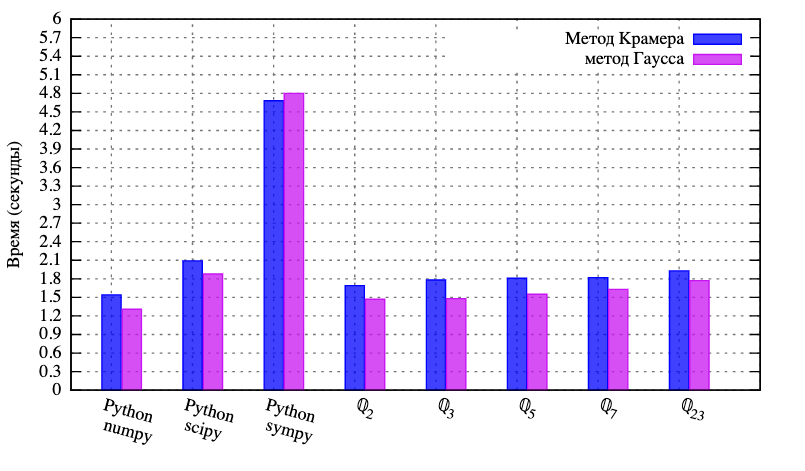
\includegraphics[width=0.95\linewidth]{../gnuplot/single/system/plot.png}}
\caption{Сравнение производительности однопоточных методов для решения СЛАУ.}
\label{img:single:system:1}
\end{figure}
\end{frame}


% Слайд 15
\begin{frame}
\frametitle{Сравнение производительности: решение СЛАУ}
\begin{figure}[H]
\centerline{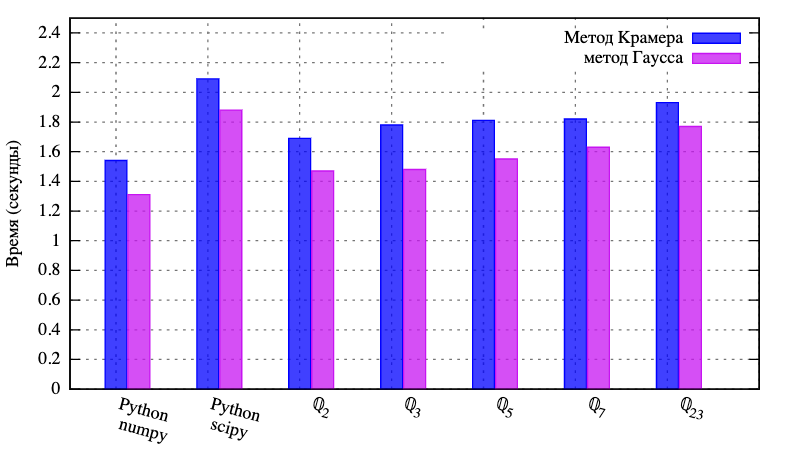
\includegraphics[width=0.95\linewidth]{../gnuplot/single/system/wosymb.png}}
\caption{Сравнение производительности однопоточных методов для решения СЛАУ (без символьного метода).}
\label{img:single:system:2}
\end{figure}
\end{frame}


% Слайд 16
\begin{frame}
\frametitle{Многопоточный алгоритм для работы с $p$-адической арифметики}
\begin{figure}[H]
\centerline{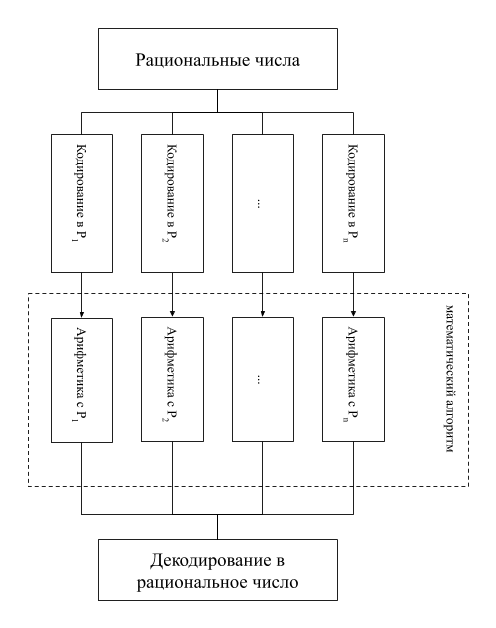
\includegraphics[width=0.5\linewidth]{images/multi/schema.png}}
\caption{Китайская теорема об остатках, скомбинированная с $p$-адической арифметикой.}
\label{img:multi:schema}
\end{figure}
\end{frame}


% Слайд 17
\begin{frame}
\frametitle{Сравнение производительности: решение СЛАУ}
\begin{figure}[H]
\centerline{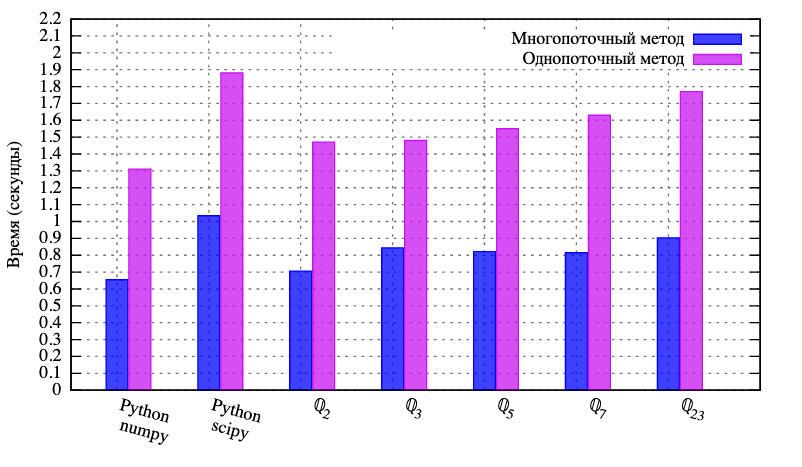
\includegraphics[width=0.95\linewidth]{../gnuplot/multi/gauss/plot.png}}
\caption{Сравнение методов для решения СЛАУ.}
\label{img:multi:gauss}
\end{figure}
\end{frame}


% Слайд 18
\begin{frame}
\frametitle{Сравнение производительности: нахождение собственных чисел и векторов (метод Якоби)}
\begin{figure}[H]
\centerline{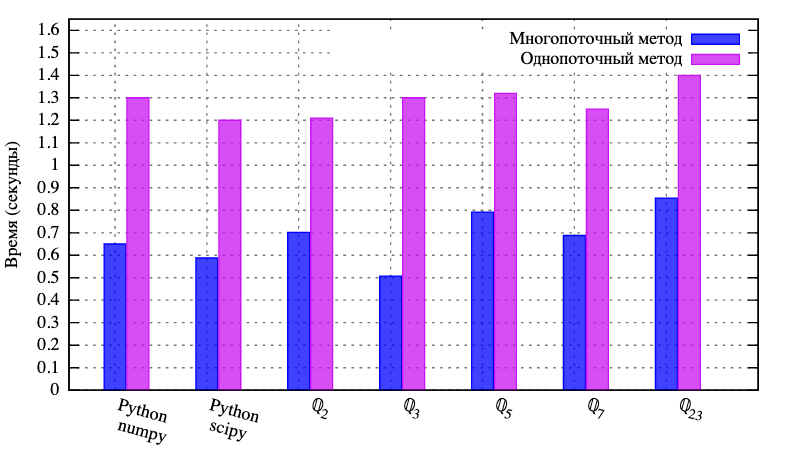
\includegraphics[width=0.95\linewidth]{../gnuplot/multi/jacoby/plot.png}}
\caption{Сравнение методов нахождения собственных чисел и собственных векторов матрицы.}
\label{img:multi:jacoby}
\end{figure}
\end{frame}


% Слайд 19
\begin{frame}
\frametitle{Сравнение производительности: нахождение собственных чисел и векторов (метод Ланцоша)}
\begin{figure}[H]
\centerline{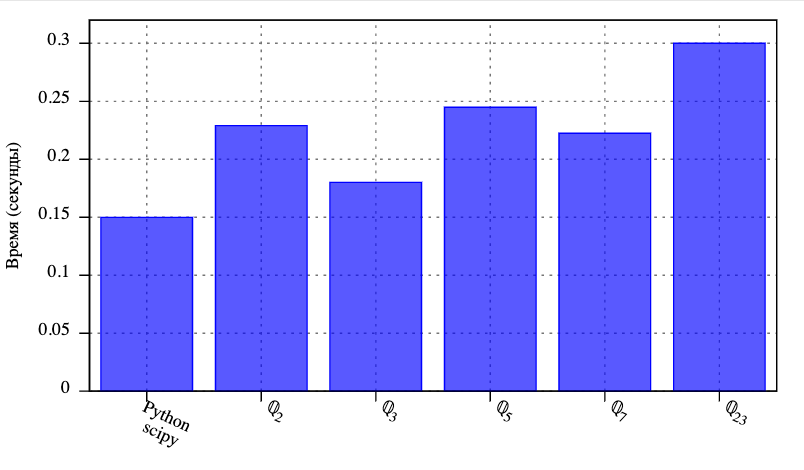
\includegraphics[width=0.95\linewidth]{../gnuplot/multi/lanczos/plot.png}}
\caption{Сравнение производительности классического и $p$-адического алгоритма Ланцоша.}
\label{img:multi:lanczos}
\end{figure}
\end{frame}


% Слайд 20
\begin{frame}
\frametitle{Сравнение производительности: решение ОДУ}
\begin{equation}
\begin{aligned}
\dfrac{\partial z}{ \partial t} = v, \\
\dfrac{\partial v}{ \partial t} = g - \alpha v^2, \\
\alpha = \frac{3\rho_f}{4\rho_k d}C_d.
\end{aligned}
\end{equation}
\noindent Аналитическое решение данного уравнения при $z(0)=0$ и $v(0)=0$ представляет собой следующие функции:

\begin{equation}
\begin{aligned}
z(t)=\frac{\log{(\cosh{(\sqrt{\alpha g} \cdot t})})}{\alpha}, \\
v(t)=\sqrt{\frac{g}{\alpha}} \cdot \tanh{(\sqrt{\alpha g} \cdot t)}.
\end{aligned}
\end{equation}
\end{frame}


% Слайд 21
\begin{frame}
\frametitle{Сравнение производительности: решение ОДУ}
В качестве физических параметров для эксперимента будем использовать параметры стандартного мяча для гольфа:
\begin{threeparttable}
\begin{longtable}[H]{lp{0.7\linewidth}}
{$d$} -- диаметр шара & 41 [мм] \\
{$\rho_k$} -- плотность сферы & 1275 [кг/м\textsuperscript{3}] \\
{$\rho_f$} -- плотность жидкости & 1.22 [кг/м\textsuperscript{3}] \\
{$C_d$} -- коэффициент трения & 0.4
\end{longtable}
\end{threeparttable}
\end{frame}


% Слайд 22
\begin{frame}
\frametitle{Сравнение производительности: решение ОДУ}
\begin{figure}[H]
\centerline{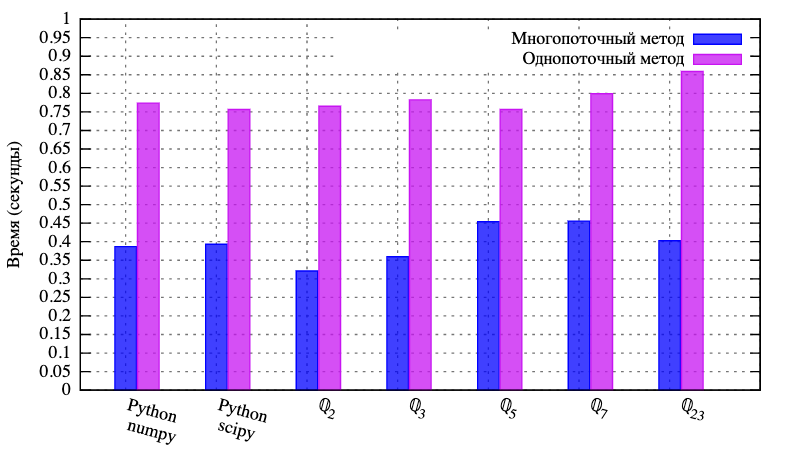
\includegraphics[width=0.95\linewidth]{../gnuplot/multi/euler/plot.png}}
\caption{Сравнение методов нахождения численного решения ОДУ с помощью метода Эйлера.}
\label{img:multi:ode:euler}
\end{figure}
\end{frame}


% Слайд 23
\begin{frame}
\frametitle{Сравнение производительности: решение ОДУ}
\begin{figure}[H]
\centerline{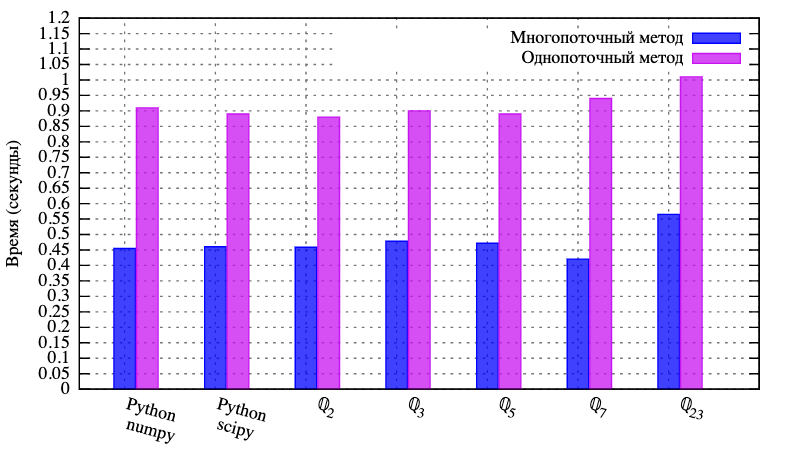
\includegraphics[width=0.95\linewidth]{../gnuplot/multi/rk/plot.png}}
\caption{Сравнение методов нахождения решения ОДУ с помощью метода Рунге-Кутты 4-го порядка.}
\label{img:comp:ode:rk}
\end{figure}
\end{frame}


% Слайд 23
%\begin{frame}
%\frametitle{Сравнение производительности: решение ОДУ}
%\begin{figure}[H]
%\centerline{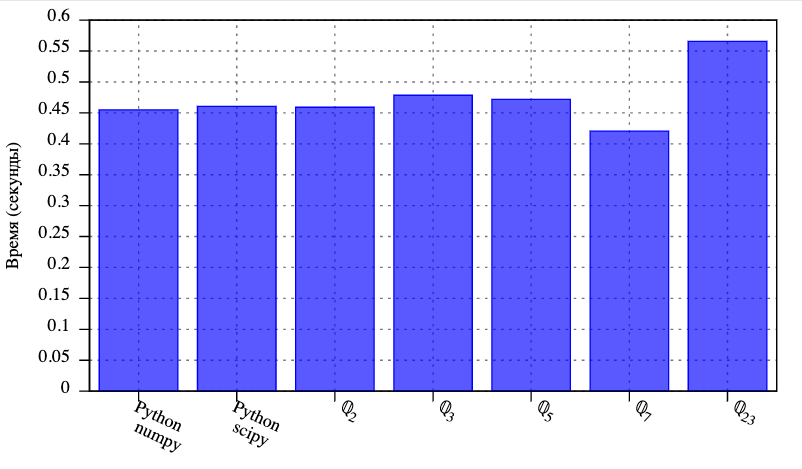
\includegraphics[width=0.95\linewidth]{../gnuplot/multi/rk/multi.png}}
%\caption{Сравнение классических методов для нахождения решения ОДУ с помощью метода Рунге-Кутты 4-го порядка и методов с использованием параллельной $p$-адической арифметики.}
%\label{img:comp:ode:rk:multi}
%\end{figure}
%\end{frame}


% Слайд 24
\begin{frame}
\frametitle{Сравнение производительности: вычисление матричной экспоненты}
\begin{defn}\label{def:exp}
Экспонентой от матрицы $A$ называется матрица

\begin{equation}
e^A=I+A+\frac{1}{2!}A^2+\cdots++\frac{1}{n!}A^n + \cdots,
\end{equation}

\noindent соответственно

\begin{equation}
e^{At}=I+tA+\frac{t^2}{2!}A^2+\cdots++\frac{t^n}{n!}A^n + \cdots.
\end{equation}
\end{defn}
\end{frame}


% Слайд 25
\begin{frame}
\frametitle{Сравнение производительности: вычисление матричной экспоненты}
\begin{figure}[H]
\centerline{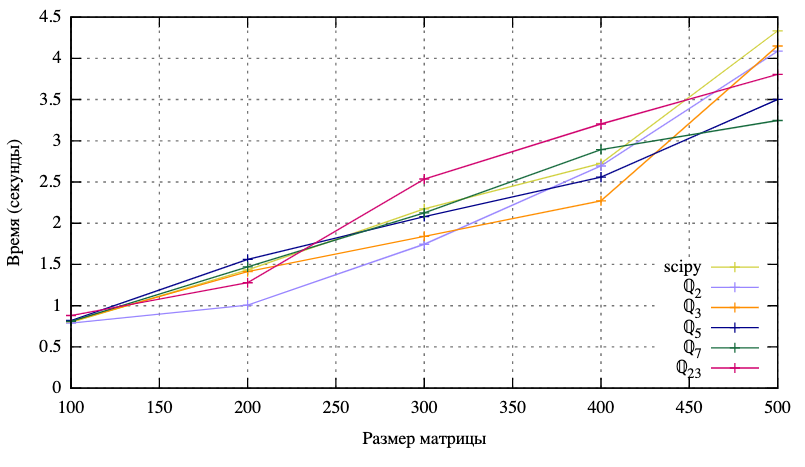
\includegraphics[width=0.95\linewidth]{../gnuplot/exp/plotfix.png}}
\caption{Сравнение классических и $p$-адических методов для вычисления матричной экспоненты.}
\label{img:exp:plot}
\end{figure}
\end{frame}


% Описание результатов курсовой работы - обязательный слайд
\begin{frame}
    \frametitle{Результаты дипломной работы}
    \begin{enumerate}
        \item Представлен программный комплекс, разработанный с использованием ЯП Python и предназначенный для осуществления операций с наиболее распространенными объектами компьютерной алгебры при использовании $p$-адической арифметики над полем $\mathbb{Q}_p$. Комплекс не имеет аналогов на ЯП Python.
        \item Произведено сравнение разработанного программного комплекса и классических методов вычислений.Тесты производительности многопоточной библиотеки показали, что что параллельная $p$-адическая арифметика сравнима с классическими методами, но, несмотря на это, является лучшей с той точки зрения, что во время вычислений не накапливает арифметическую ошибку.
    \end{enumerate}    
\end{frame}

\begin{frame}[allowframebreaks]
\frametitle{Список использованных источников}
\nocite{*}
\bibliographystyle{biblio/ugost}
\bibliography{biblio/biblio}
\end{frame}


\begin{frame}[c]
\begin{center}
\frametitle{\LARGE Спасибо за внимание!}

{\LARGE \inserttitle}

\bigskip\bigskip

{\large \insertauthor}

\bigskip\bigskip

{\insertinstitute}

\bigskip\bigskip

{\large \insertdate}
\end{center}
\end{frame}

\end{document}